% Figure 2: Multi-scale agency (Levin CLC) + Synthesis diagram

\begin{figure*}[!t]
\centering

\begin{minipage}[t]{0.48\textwidth}
\centering
{\small\bfseries C.\enspace Kognitiv lyskjegle (CLC)}\\[4pt]
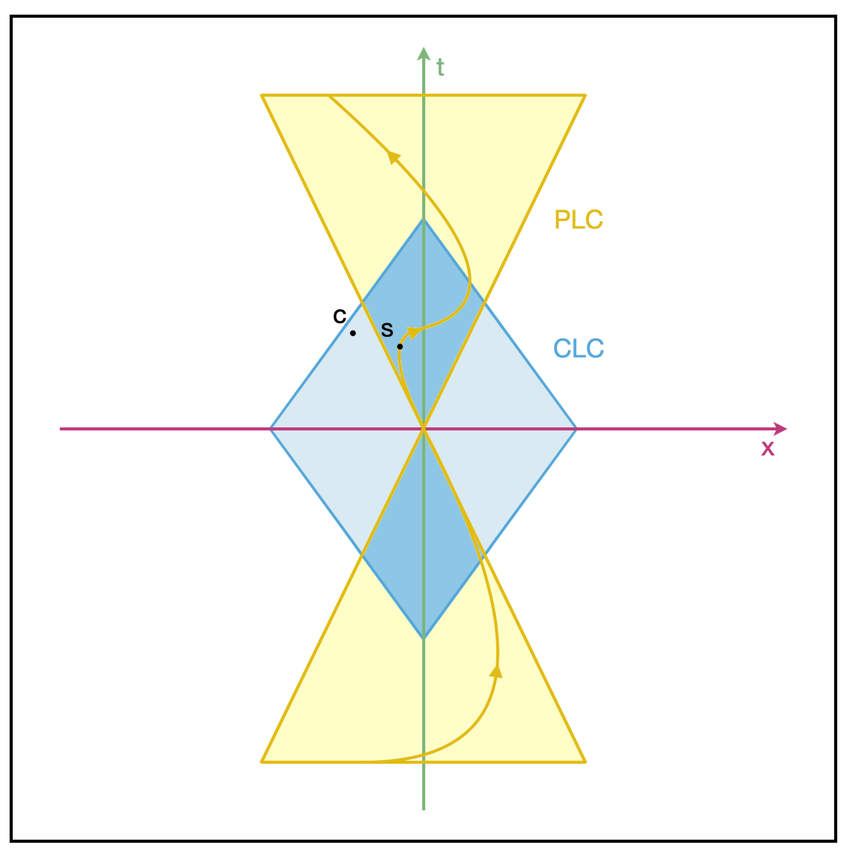
\includegraphics[width=0.85\textwidth]{figures/levin-clc-boundary.png}
\end{minipage}%
\hfill
\begin{minipage}[t]{0.48\textwidth}
\centering
{\small\bfseries D.\enspace Syntesen}\\[4pt]
\includegraphics[width=0.85\textwidth]{figures/syntese_diag.png}
\end{minipage}

\caption{\textbf{C}: Ein agent si omsorgskjegle (CLC, blått) innanfor den fysiske lyskjegla (PLC, gult). Omsorgsdimensjonaliteten $\dim C(A)$ avgjer kva del av landskapet agenten kan representere. Frå \textcite{Doctor2024}. \textbf{D}: Syntese-likninga: tre kjeldetradisjonar konvergerer i kjerne-likninga; stipla pil viser $K$-ekspansjonstilbakekopling.}
\label{fig:agency-synthesis}
\end{figure*}
